\chapter{Combat}\label{chap:combat}
\section{Introduction to Combat}
Combat is a staple of most RPGs. 
It's intense, often exhilarating, and it gives the players a chance to strategise.
Combat is essentially a series of \textit{Contests of Skill} (see Section~\ref{sec:contest}), but due to the nature of combat are naturally a bit more involved.
\subsection{Turns}
Combat is split into a number of turns, each turn represents about 6 seconds of in-game time, meaning 10 turns make up an in-game minute.

\paragraph{Note} One turn is the time it takes for every character to have had a go, not the time for each individual character.
\subsection{Turn Order}
To determine turn order, each player rolls $1d6+Athletics$. The turn-order is then ordered highest to lowest. Highest result goes first, lowest goes last. Any ties require a re-roll.

\paragraph{Example} Alice, Bob, and Clarice all roll for turn order. They have an athletics score of 9, 9, and 10 respectively. Alice rolls a 5, Bob rolls 3, and Clarice rolls a 6. Clarice goes first with 16, Alice is next with 14, and Bob is last with a score of 12.

\subsection{Movement}\label{sec:movement}
Particularly, the characters rely on their movement points to move about the battle mat.
Movement is 8-directional (see Figure~\ref{fig:directions}), and moving in any direction costs 1 movement point.

\begin{figure}
    \centering
    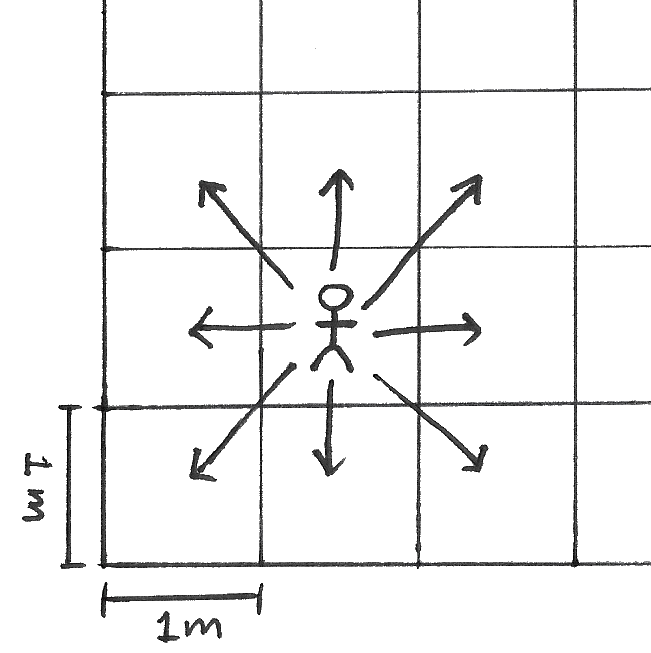
\includegraphics{graphics/directions-trans.png}
    \caption{The eight movement directions}
    \label{fig:directions}
\end{figure}

Your character can only move as far as their movement points allow, but you may choose to move a shorter distance if you so desire.
Figure~\ref{fig:movement} shows an example of a character moving 4 squares, which is worth 4 movement points.

\begin{figure}
    \centering
    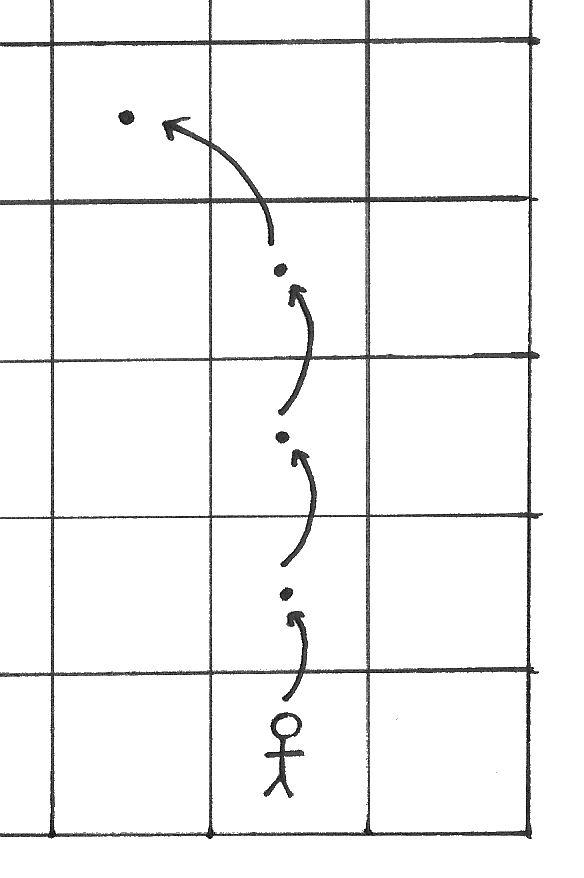
\includegraphics{graphics/movement-trans.png}
    \caption{Example of movement.}
    \label{fig:movement}
\end{figure}

\subsection{The Grid}
The battle mat is subdivided into a grid of squares. 
The in-game size of a square is $1m^2$, although the GM may scale it up or down as necessary.
The GM must alert the players of the scale if it differs from the standard $1m^2$.

\newpage
\subsection{Phases}\label{sec:phases}
Turns in Siren is split into two distinct phases: \textit{Proactive} and \textit{Reactive}.

The phases are structured as follows:
\begin{enumerate}
  \item Proactive 
  \item Reactive
  \item Damage Calculation (if applicable)
\end{enumerate}

\subsubsection{Proactive Phase}
The proactive phase is what you would think of as ``your turn'', during your proactive phase you can pick any two of the following actions: \textit{Moving}, \textit{Bracing}, or \textit{Attacking}.
If however, your character is performing a non-combat action (such as picking a lock), this takes up the entire proactive phase.

\paragraph{Move}
Movement means your character can move up to half their speed-rating.

\paragraph{Brace}
Your character takes a defensive stance and gets $+2$ to any defence rolls this turn.

\paragraph{Attack}
You character gets to roll an attack.

If your character performs a ranged attack, you need to check the weapon's range.
The skill check to attack is done at $-3$ for every time the range of the weapon is exceeded.

\paragraph{Ranged Attack Example} Will the Ranger is out hunting for his party. He spots a deer in the distance. His bow has a range of 100 metres, the deer is 300 metres away. This exceeds the bow's range twice ($2\times -3$ penalty). Will must roll $Longbow-6$ to succeed.

\paragraph{Note} In the proactive phase, your character can pick the same option twice.

\subsubsection{Reactive Phase}
When your character is being attacked, they enter the reactive phase.
During this phase, you can choose any \textbf{one} of either \textit{Moving}, \textit{Defending}, \textit{Counter-Attacking}
\paragraph{Move}
Movement means your character can move up to half their speed-rating.
\paragraph{Defend}
Your character is able to perform a defensive roll + any cumulative modifiers from their previous proactive phase.

Note that this means if you didn't move or brace yourself in the previous turn, you don't get the relevant bonuses.
\paragraph{Counter-Attack}
Instead of moving or defending, you may simply initiate an attack in response.

\section{Taking Damage}
It's not uncommon that you take damage during combat.
After all, having an angry wizard throw fireballs at you is going to hurt!
This section describes the ways in which damage is taken, and what the consequences are.
See Chapter~\ref{chap:defence} for more info about damage resistance.

\subsection{Health Points (HP)}\label{sec:health-points}
Every character has a number of Health Points (HP).
The amount of HP a player has determines the player's level of consciousness:

\begin{center}
  \begin{tabular}{r | l}
    \textbf{HP Left} & \textbf{Effect} \\\hline
    $HP > 0$         & Alive and able to fight. \\
    $HP \leq 0$      & Roll against $2 \times Con$ to see if you faint. \\
    $HP \leq -MaxHP$ & Roll against $2 \times Con$ to see if you die.
  \end{tabular}
\end{center}

\paragraph{Note} Rolling against your $HP$ happens at the start of your turn.
  
\subsection{Fatigue Points (FP)}\label{sec:fatigue-points}
Fatigue is a different kind of damage.
One that affects you character more directly.
There are many different sources of fatigue: heat, starvation, dehydration, sleep deprivation, etc.

For every point of Fatigue lost, your character suffers a $-1$ penalty on all skill rolls.

\begin{center}
  \begin{tabular}{r | l}
    \textbf{FD Taken} & \textbf{Effect} \\\hline
    $FP \leq MaxFP/2$ & Roll against $MaxFP - FP$ to see if you faint. \\
    $FP \leq MaxFP$   & Immediately faint from exhaustion.
  \end{tabular}
\end{center}

\paragraph{Example} Charles has been walking the desert for the past five days.
The heat is getting to him, and he's lost 5 points of FP.
Charles has 10 FP, but due to the damage, he needs to roll 5 or less to not faint in the sand.
He rolls 9 and immediately collapses.

\section{Healing Damage}
Healing usually takes place \textit{outside} of combat, but can also be performed during combat as a \textit{Long Action}.
Healing takes time, and depending on the severity of the wound, the healing process takes a different amount of time.

The skill used for healing entirely depends on the task at hand.
Surgeries, anæsthetics, medicine, therapy, etc. all fall under the \textit{Academics} skill, while caretaking falls under \textit{Nursing}.
If however, it's automatic, then it depends on the effectiveness of that particular remedy.
That is, applying bandages or stitching a wound depends on the skill of the doer, while drinking a magic potion is dependent on the strength of the potion.

Healing comes in three different variants:

\begin{center}
  \begin{itemize}
  \item \textbf{Healing by mending.}
    This is the slowest form of healing, refers to any kind of healing performed via bandages, stitches, rest, or similar.\\
    Mending happens over the course of days or weeks.
  \item \textbf{Healing by potion.}
    The second-fastest form of healing, which refers to injecting or ingesting a substance that has regenerative properties. \\
    Potions heal over the course of minutes or hours.
  \item \textbf{Healing by magic.}
    The fastest form of healing, which refers to any procedure that facilitates instant healing, magic or otherwise.
  \end{itemize}
\end{center}

\paragraph{Note} Healing refers to both healing Health and Fatigue.
A cup of coffee, for example, is a fatigue-healing potion that takes about 15 in-game minutes to kick in.
